\documentclass[12p,a4paper]{article}
\usepackage[utf8]{inputenc}
\usepackage[T1]{fontenc,url}
\usepackage{multicol}
\usepackage{multirow}
\usepackage{parskip}
\usepackage{lmodern}
\usepackage{microtype}
\usepackage{verbatim}
\usepackage{amsmath, amssymb}
\usepackage{tikz}
\usepackage{physics}
\usepackage{mathtools}
\usepackage{algorithm}
\usepackage{algpseudocode}
\usepackage{listings}
\usepackage{enumerate}
\usepackage{graphicx}
\usepackage{float}
\usepackage{hyperref}
\usepackage{tabularx}
\usepackage{siunitx}
\usepackage{fancyvrb}
\usepackage[makeroom]{cancel}
\usepackage[margin=2cm]{geometry}
\renewcommand{\baselinestretch}{1}
\renewcommand{\b}{\boldsymbol}
\newcommand{\h}{\hat}
\newcommand{\m}{\mathbb}
\renewcommand{\exp}{e^}
\newcommand{\half}{\frac{1}{2}}
\newcommand{\eE}{\langle E \rangle}
\setlength\parindent{0pt}


\begin{document}
\section*{Part 1}
\subsection*{a)}
The partition function is the sum of the Boltzmann factors of all possible states, giving
\begin{align*}
    Z = \sum\limits_s \exp{-E(s)/kT} = 3\exp{-2\epsilon/kT} + \exp{-\epsilon/kT} = \exp{-\epsilon/kT}\qty[3\exp{\epsilon/kT} + 1]
\end{align*}



\subsection*{b)}
The average energy, or expectation value of the energy, is defined from the partition function as
\begin{align*}
    \eE &= \frac{1}{Z} \sum\limits_s E(s)\exp{-E(s)/kT} = \qty(\frac{1}{\exp{-\epsilon/kT}\qty[3\exp{\epsilon/kT} + 1]})\cdot\qty(2\epsilon 3\exp{-2\epsilon/kT} + \epsilon\exp{-\epsilon/kT}) \\ \\
    &= \frac{\epsilon\exp{-\epsilon/kT}}{\exp{-\epsilon/kT}} \cdot \frac{6\exp{-\epsilon/kT} + 1}{3\exp{-\epsilon/kT} + 1}
    = \epsilon\frac{6\exp{-\epsilon/kT} + 1}{3\exp{-\epsilon/kT} + 1} = 2\epsilon - \frac{\epsilon}{3\exp{-\epsilon/kT} + 1}
\end{align*}
Giving us an expression for the expectation value of the energy, as function of temperature
\begin{align}\label{eqn:eE}
    \eE = 2\epsilon - \frac{\epsilon}{3\exp{-\epsilon/kT} + 1}
\end{align}


\subsection*{c)}
The heat capacity is, for a given volume and number of particles, given as
\begin{align*}
    C_V = \qty(\frac{\partial E}{\partial T})_{N,V}
\end{align*}
Applying this to our expression for the average energy, \ref{eqn:eE}, we get
\begin{align*}
    C_V = \frac{\partial \eE}{\partial T} = \frac{\partial}{\partial T}\qty(2\epsilon - \frac{\epsilon}{3\exp{-\epsilon/kT} + 1})
    = \epsilon\frac{\partial}{\partial T}\qty(\frac{1}{3\exp{-\epsilon/kT} + 1})
\end{align*}
Substituting $u = 3\exp{-\epsilon/kT} + 1$, gives
\begin{align*}
    C_V = \epsilon\frac{\partial}{\partial u}\qty(\frac{1}{u}) \cdot \frac{\partial u}{\partial T}
    = -\epsilon\frac{1}{u^2} \cdot \frac{\partial}{\partial T}\qty(3\exp{-\epsilon/kT} + 1)
\end{align*}
again, substituting $v = -\epsilon/kT$ in the last derivative, gives
\begin{align*}
    C_V = -\epsilon\frac{1}{u^2} \cdot \frac{\partial}{\partial v}3e^v \cdot \frac{\partial}{\partial T}\qty(\frac{-\epsilon}{kT})
    = -\epsilon\frac{1}{u^2} \cdot 3e^v \cdot \frac{\epsilon}{kT^2}
\end{align*}
Inserting for $u$ and $v$ gives
\begin{align*}
    C_V = -\epsilon\frac{1}{(3\exp{-\epsilon/kT} + 1)^2} \cdot 3\exp{-\epsilon/kT} \cdot \frac{\epsilon}{kT^2}
    = -\frac{3\epsilon^2 \exp{-\epsilon/kT}}{(3\exp{-\epsilon/kT} + 1)^2 kT^2}
\end{align*}
At last giving us the heat capacity as function of temperature
\begin{align}\label{eqn:C_V}
    C_V = -\frac{3\epsilon^2 \exp{-\epsilon/kT}}{(3\exp{-\epsilon/kT} + 1)^2 kT^2}
\end{align}

Figure \ref{fig:C_V} shows heat capacity as a function of temperature between 0 and 300 Kelvin. The energy $\epsilon$ was decided purely experimentally, to give reasonable graphs. The Boltzmann constant was set to it's usual value of $1.38\cdot 10^{-23}$.

For each $\epsilon$, we see that the heat capacity starts at 0, before rapidly expanding to some maximum value. It thereafter falls more slowely off, going towards 0 at higher temperatures. It seems that at really low and high temperatures, there is virtually no net energy gained from increasing the temperature.

\begin{figure}[H]
    \centering
    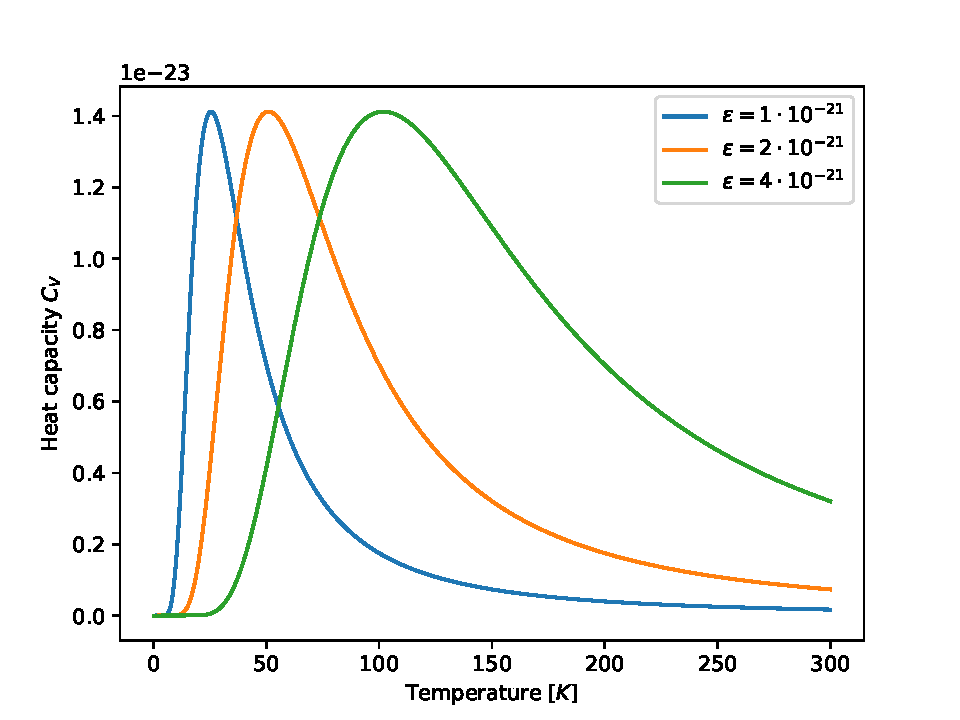
\includegraphics[width=0.6\textwidth]{taskc.pdf}
    \caption{}
    \label{fig:C_V}
\end{figure}




\section*{Part 2}
\subsection*{d)}
The partition function over all states $s$ is still given as
\begin{align*}
    Z = \sum\limits_s \exp{-E(s)/kT}
\end{align*}
Instead of summing over all the states, we can sum over the different energy-levels. We must then account for the degeneracy of the energy-levels (energy levels that appear in multiple states).
\begin{align}\label{eqn:Z_R}
    Z_R = \sum\limits_j g(j) \exp{-\epsilon_j/kT} = \sum\limits_j (2j + 1)  \exp{-j(j+1)\theta_r/T}
\end{align}



\subsection*{e)}
We will take a look at the terms $z(j)$ in the partition function:
\begin{align*}
    z(j) = (2j + 1)  \exp{-j(j+1)\theta_r/T}
\end{align*}

For the $T/\theta_r >> 1$ case, we see that we get a Boltzmann-looking distribution, where the most likely energy state is somewhere around 20 in our case, and falling off towards 0 and higher values.

For the $T/\theta_r << 1$ case, we see that only the ground state contributes to the parition function, and is the absolute most probable state to find the system in.

This all makes sense, as the more energy is avaliable to the system (through $T$), the higher the expected energy-state. $\theta_r$ must be some parameter inversely effecting this, like how far there is between the different energy-levels.

\begin{figure}[H]
    \centering
    \includegraphics[width=0.6\textwidth]{{taske_1}.pdf}
    \includegraphics[width=0.6\textwidth]{{taske_2}.pdf}
    \includegraphics[width=0.6\textwidth]{{taske_3}.pdf}
\end{figure}
\newpage


\subsection*{f)}
In the limit $T >> \theta_r$, the probability will be distributed among very many energy-states ($j$). This means that the $z(j)$ curve will be very smooth, and we can consider the sum to be a Riemann sum. By this logic, we can approximate it as the intergral:
\begin{align*}
    Z_R = \sum\limits_j (2j + 1)  \exp{-j(j+1)\theta_r/T} \approx \int\limits_0^{\infty} (2j + 1)  \exp{-j(j+1)\theta_r/T} dj
\end{align*}
Substituting $u = j(j+1)$, we have $\frac{d u}{d j} = 2j+1$ , giving $d j = \frac{du}{2j + 1}$. Inserting this gives
\begin{align*}
    Z_R = \int\limits_0^{\infty} \exp{-u\theta_r/T} du = \qty[-\frac{T}{\theta_r}\exp{-u\theta_r/T}]_0^{\infty} = \frac{T}{\theta_r}
\end{align*}



\subsection*{g)}
Looking back at our definition of $Z_R$ \ref{eqn:Z_R}, we can write it out as
\begin{align}\label{eqn:E_low}
    Z_R = 1 + 3\exp{-2\theta_r/T} + ...
\end{align}
All terms but the first fall off incredibly quickly in the case $T/\theta_r << 1$. $Z_R$ will converge quickly to 1.



\subsection*{h)}
In the high-energy limit, we can use the approximation
\begin{align*}
    \eE = -\frac{1}{Z}\frac{\partial Z}{\partial \beta} = -\frac{1}{Z}\frac{\partial Z}{\partial \beta}
\end{align*}
for $\beta = 1/kT$. We use the high-energy approximation of $Z_R$, $Z_R =\frac{T}{\theta_r} = \frac{1}{\beta k \theta_r}$:
\begin{align*}
    \eE = \beta k \theta_r \frac{1}{\beta^2 k \theta_r} = \frac{1}{\beta} = kT
\end{align*}
According to the equipartition theorem, this corresponds to the energy of a system with two degrees of freedom.

In the low-energy limit, we use our low-energy approximation of $E$ \ref{eqn:E_low}, and insert it into the definition of average energy:
\begin{align*}
    \eE = \frac{1}{Z}\sum\limits_s E(s)\exp{-\beta E(s)} = \frac{1}{1 + 3\exp{-2\theta_r/T}} \cdot  6\theta_r k \exp{-2\theta_r/T}
    = \frac{6\theta_r k \exp{-2\theta_r/T}}{1+3\exp{-2\theta_r/T}}
\end{align*}
This will as expected run towards 0 in the limit $T/\theta_r << 1$.



\subsection*{i)}
The definition of heat capacity is still $C_V = \qty(\frac{\partial E}{\partial T})_{N,V}$

For our high-temperature definition of $E$, we get the heat capacity
\begin{align*}
    C_V = \frac{\partial}{\partial T}(kT) = k
\end{align*}

For our low-temperature definition of $E$, we get
\begin{align*}
    C_V = \frac{\partial}{\partial T}\qty(\frac{6\theta_r k \exp{-2\theta_r/T}}{1+3\exp{-2\theta_r/T}})
\end{align*}
which evaluates to
\begin{align*}
    C_V = \frac{12\theta_r^2k\exp{-2\theta_r/T}}{T^2(1+3\exp{-2\theta_r/T})^2}
\end{align*}



\subsection*{j)}
I've taken a somewhat lazy approach, and simply used the high-energy approximation of $Z_R$ for large $T/\theta_r$ values, and the actual definition of $Z_R$ for smaller values. I set the limit between these cases to $T/\theta_r > 10^6$, although this is a somewhat arbitrary choice. For values $T/\theta_r < 10^6$, I simply sum all $j$-values up to $10^6$, because this is a rather light workload for such sizes.


\subsection*{k)}
Below we see a logaritmic plot of the partition function over a range of $T/\theta_r$ values. Note how there is no visible dicontinuity at $T/\theta_r = 10^6$, where the limit between our two calculation methods lie.
\begin{figure}[H]
    \centering
    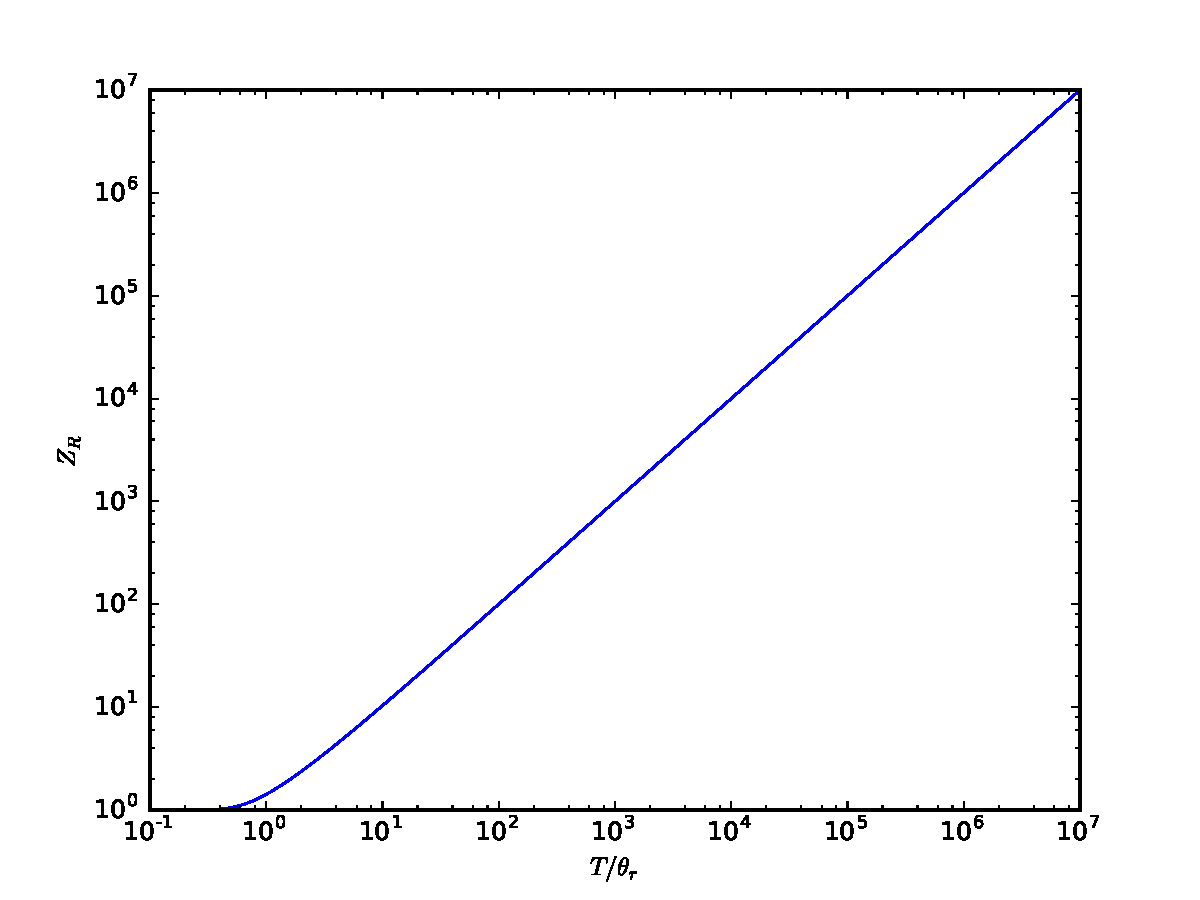
\includegraphics[width=0.6\textwidth]{taskj.pdf}
\end{figure}



\subsection*{l)}
If we look at what value our function gives while still using the exact $Z_R$ function, we get
\begin{verbatim}
    print(Z(1e6))
    >>> 1000000.33333
\end{verbatim}
The estimated value from our high-energy case would be $Z_R = T/\theta_r = 100000$. We see we're off by a factor around $10^6$ - $10^7$. This is due to estimating the sum as an integral, which is only accurate when $T/\theta_r \rightarrow \infty$.



\subsection*{m)}
We can find the expectation value of the energy by calculating the partition function with and without the energy weight, and taking the ratio:
\begin{align*}
    E = \frac{\sum \epsilon_j z(j)}{\sum z(j)} = \frac{\sum j(2j+1)(j+1)\theta_r k\exp{-j(j+1)\theta_r/T_i}}{\sum (2j+1)\exp{-j(j+1)\theta_r/T_i}}
\end{align*}

Since the heat capacity is nothing but the temperature-derivative of energy, we can use a derivation scheme, to numerically calculate it:
\begin{align*}
    C_V(T_i) = \frac{E(N, V, T_{i+1}) - E(N, V, T_i)}{T_{i+1} - T_i}
\end{align*}


\section*{Appendix - Code}
\subsection*{Task c}
\verbatiminput{taskc.py}
\subsection*{Task e}
\verbatiminput{taske.py}
\newpage
\subsection*{Task j}
\verbatiminput{taskj.py}


\end{document}
